% =====================================================================
\section{The Tahawus function}\label{sec:function}
% =====================================================================

Throughout, $x^{x}$ is understood as $\exp(x \ln x)$ for $x > 0$.

\begin{definition}[forward map and Tahawus function]\label{def:tah}
Let
\begin{equation}\label{eq:f-def}
    f(x) \;:=\; \frac{x^{x} - 1}{x} \;=\; x^{x-1} - \frac{1}{x},
    \qquad x > 0 .
\end{equation}
The \emph{Tahawus function} is the compositional inverse of $f$,
\begin{equation}\label{eq:tah-def}
    \Tah \;:=\; f^{-1},
\end{equation}
so that $y = f(x) \iff x = \Tah(y)$, i.e.
\begin{equation}\label{eq:defining}
    \Tah(y)^{\,\Tah(y)} \;=\; y\,\Tah(y) + 1 .
\end{equation}
\end{definition}

The domain of definition is settled by the following theorem, which
also shows that the super-quadratic \eqref{eq:superquad} has exactly one
positive solution for every real $b$. The proof rests on a single
elementary inequality, isolated as a lemma.

\begin{lemma}\label{lem:mono}
For every $0 < x < 1$,
\begin{equation}\label{eq:phi-ineq}
    \Phi(s) \;:=\; \ee^{-s\ee^{-s}}\bigl(1 + (s-1)\ee^{-s}\bigr) \;<\; 1,
    \qquad s := -\ln x > 0 .
\end{equation}
\end{lemma}

\begin{proof}
Put $t := (s-1)\ee^{-s}$. The map $h(s) = (s-1)\ee^{-s}$ satisfies
$h(0) = -1$ and $h'(s) = (2-s)\ee^{-s} > 0$ for $0 < s < 2$, so $h$ is
strictly increasing from $-1$ on $(0,2)$ and satisfies $h(s) \ge 0$ for
$s \ge 1$; in particular $t > -1$ for all $s > 0$. Since
$\ln(1+t) \le t$ for $t > -1$, with equality only at $t = 0$,
\[
    \ln \Phi(s)
    \;=\; -s\ee^{-s} + \ln\bigl(1 + (s-1)\ee^{-s}\bigr)
    \;\le\; -s\ee^{-s} + (s-1)\ee^{-s}
    \;=\; -\ee^{-s} \;<\; 0 ,
\]
and the inequality is strict because the final term $-\ee^{-s}$ is
strictly negative. Hence $\Phi(s) < 1$.
\end{proof}

\begin{theorem}[the Tahawus function is a well-defined analytic
order isomorphism]\label{thm:bijection}
The map $f$ of \eqref{eq:f-def} is real-analytic and strictly
increasing on $(0,\infty)$, with
\[
    \lim_{x \to 0^{+}} f(x) = -\infty,
    \qquad
    \lim_{x \to +\infty} f(x) = +\infty .
\]
Consequently $f$ is a bijection $(0,\infty) \to \R$, and $\Tah \colon
\R \to (0,\infty)$ is a strictly increasing real-analytic bijection.
In particular, for every real $b$ the super-quadratic
$x^{x} = bx + 1$ has exactly one positive solution, namely
$x = \Tah(b)$.
\end{theorem}

\begin{proof}
Differentiating \eqref{eq:f-def},
\begin{equation}\label{eq:fprime}
    f'(x) \;=\; x^{x-1}\Bigl(\ln x + 1 - \frac{1}{x}\Bigr) + \frac{1}{x^{2}} ,
\end{equation}
so that, multiplying by $x^{2}$,
\begin{equation}\label{eq:x2fprime}
    x^{2} f'(x) \;=\; x^{x}\bigl(x \ln x + x - 1\bigr) + 1 .
\end{equation}
For $x \ge 1$ both terms on the right are nonnegative ($x\ln x \ge 0$,
$x - 1 \ge 0$), so $f'(x) \ge x^{-2} > 0$. For $0 < x < 1$, write
$x = \ee^{-s}$ as in Lemma~\ref{lem:mono}; then
\[
    x^{x}\bigl(x\ln x + x - 1\bigr)
    \;=\; \ee^{-s\ee^{-s}}\bigl(1 + (s-1)\ee^{-s}\bigr)
    \;=\; \Phi(s) \;<\; 1
\]
(the first equality is a direct substitution of $x = \ee^{-s}$:
$x^{x} = \ee^{-s\ee^{-s}}$ and $x\ln x + x - 1 = \ee^{-s}(1 - s) + 
\ee^{-s} - 1 = -(1 + (s-1)\ee^{-s})$). Hence $x^{2}f'(x) = 1 - \Phi(s)
> 0$, and $f$ is strictly increasing on all of $(0,\infty)$.

For the limits: since $\ee^{u} = 1 + u + O(u^{2})$ as $u \to 0$ and
$x \ln x \to 0$ as $x \to 0^{+}$,
\[
    f(x) \;=\; \frac{x^{x} - 1}{x} \;=\; \ln x + O\bigl(x \ln^{2} x\bigr)
    \;\longrightarrow\; -\infty ,
\]
while for $x \ge 2$, $x^{x-1} \ge x$ (i.e.\ $x^{x-2} \ge 1$), so
$f(x) = x^{x-1} - x^{-1} \ge x - 1 \to +\infty$. Real-analyticity of
$f$ on $(0,\infty)$ is clear ($x \mapsto \exp(x\ln x)$ is
real-analytic there), and since $f' > 0$ everywhere, the inverse
function theorem makes $\Tah$ real-analytic on $\R = f\bigl((0,\infty)\bigr)$,
with
\[
    \Tah'(y) \;=\; \frac{1}{f'\bigl(\Tah(y)\bigr)} \;>\; 0 .
    \qedhere
\]
\end{proof}

\begin{corollary}[exact values, monotonicity in the parameter]
\label{cor:values}
The map $b \mapsto \Tah(b)$ is strictly increasing, and
\[
    \Tah(0) = 1, \qquad
    \Tah\Bigl(\frac{n^{n}-1}{n}\Bigr) = n \quad (n \in \N),
\]
in particular $\Tah\bigl(\tfrac{3}{2}\bigr) = 2$,
$\Tah\bigl(\tfrac{26}{3}\bigr) = 3$. The Tahawus constant
$\alpha := \Tah(1)$ is the unique positive root of $x^{x} = x + 1$ and
lies in $(1,2)$.
\end{corollary}

\begin{proof}
$f(n) = (n^{n}-1)/n$ by definition, and $f(1) = 0 < 1 < f(2) =
\tfrac32$, so $\alpha = \Tah(1) \in (1,2)$. Everything else is
immediate from Theorem~\ref{thm:bijection}.
\end{proof}

Figure~\ref{fig:mirror} shows $f$ and $\Tah$ as mirror images across the
diagonal. Three features deserve attention, and all three are made
precise in the remainder of the paper: the crossing at the reflected
pair of points $(1,0)$ and $(0,1)$, at which both curves are tangent to
lines of slope $1$ (the lines $y = x \mp 1$); the exponential approach
of $\Tah$ to $0$ as $y \to -\infty$; and the logarithm-like growth on
the right.

\begin{figure}[t]
    \centering
    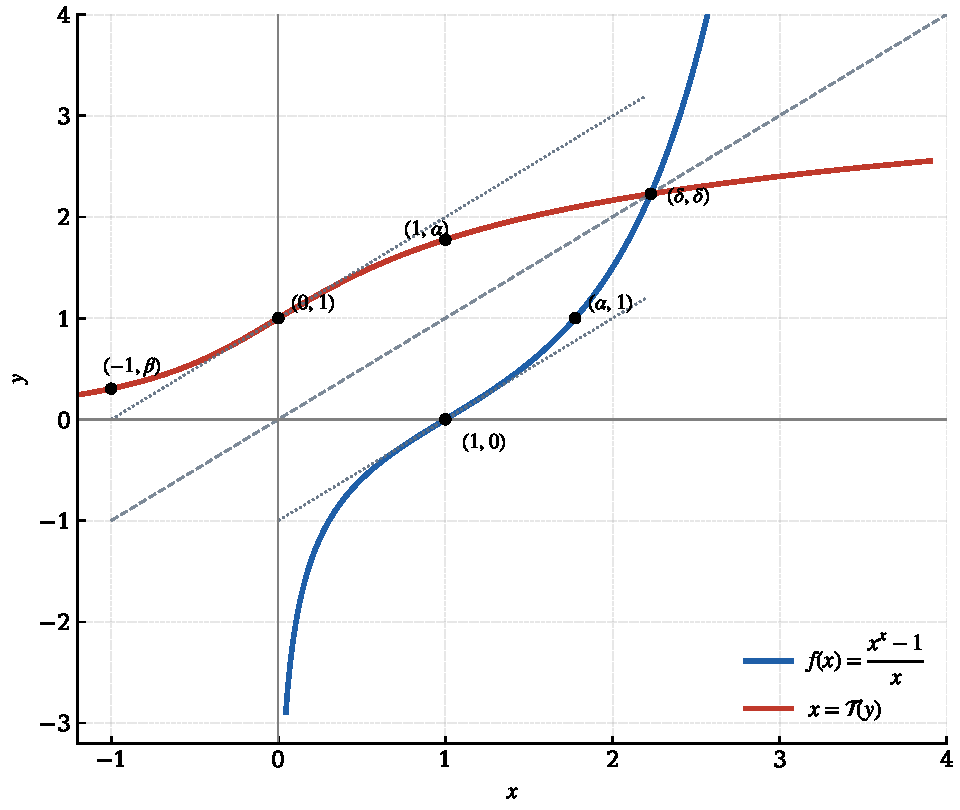
\includegraphics[width=0.78\textwidth]{figures/fig1_mirror.pdf}
    \caption{The forward map $f(x) = (x^{x}-1)/x$ (blue) and the Tahawus
    function $\Tah$ (red), mirror images across the diagonal (dashed).
    Dotted lines: the common tangent directions $y = x \mp 1$ at the
    reflected pair $(1,0)$--$(0,1)$. Marked points include
    $\alpha = \Tah(1)$, $\beta = \Tah(-1)$ and the fixed point
    $\delta$ of Section~\ref{sec:dynamics}.}
    \label{fig:mirror}
\end{figure}

\begin{proposition}[first derivatives and the reflected inflection]
\label{prop:derivatives}
Let $u := x - 1$. Then
\begin{equation}\label{eq:f-series}
    f(1+u) \;=\; u + \frac{u^{3}}{2} - \frac{u^{4}}{6} + \frac{u^{5}}{4} -
    \frac{7u^{6}}{40} + O(u^{7}) ,
\end{equation}
and consequently
\[
    f'(1) = 1,\qquad f''(1) = 0,\qquad f'''(1) = 3,\qquad f''''(1) = -4,
\]
while for the inverse function,
\[
    \Tah(0) = 1,\quad
    \Tah'(0) = 1,\quad
    \Tah''(0) = 0,\quad
    \Tah'''(0) = -3,\quad
    \Tah''''(0) = 4 .
\]
Both $f$ and $\Tah$ have an inflection at the reflected pair
$(1,0)$, $(0,1)$, with common tangent directions of slope exactly $1$.
\end{proposition}

\begin{proof}
Expanding $(1+u)\ln(1+u) = u + \tfrac{u^{2}}{2} - \tfrac{u^{3}}{6} +
\tfrac{u^{4}}{12} - \cdots$ and exponentiating,
\[
    (1+u)^{1+u} \;=\; 1 + u + u^{2} + \frac{u^{3}}{2} + \frac{u^{4}}{3} +
    O(u^{5}) ,
\]
whence, dividing by $1+u$,
\[
    \frac{(1+u)^{1+u} - 1}{1+u}
    \;=\; u + \frac{u^{3}}{2} - \frac{u^{4}}{6} + \frac{u^{5}}{4} -
    \frac{7u^{6}}{40} + O(u^{7}) ,
\]
(the quadratic term cancels). The derivative statements for $f$ follow
by comparing coefficients, since $f'(1+u) = 1 + \tfrac32 u^{2} -
\tfrac{2}{3}u^{3} + O(u^{4})$ shows $f''(1) = 0$ directly. For the
inverse, use $\Tah'(0) = 1/f'(1) = 1$,
$\Tah''(y) = -f''(x)/f'(x)^{3}$ and
$\Tah'''(y) = -f'''(x)/f'(x)^{3} + 3f''(x)^{2}/f'(x)^{5}$
(evaluated at $x = \Tah(y)$, all at $x = 1$), giving $\Tah'''(0) = -3$;
the value $\Tah''''(0) = 4$ is read off the reversion series of
Theorem~\ref{thm:maclaurin}. The inflection claim follows from
$f''(1) = 0 < f'''(1)$ and its mirrored statement, and the tangent
lines are $y = x - 1$ (for $f$ at $(1,0)$) and its reflection
$y = x + 1$ (for $\Tah$ at $(0,1)$).
\end{proof}

% =====================================================================
\section{The Tahawus constant: transcendence and arithmetic}
\label{sec:constant}
% =====================================================================

With the function firmly in place we turn to arithmetic. The key
observation is that the equation $x^{x} = bx+1$ is \emph{irrationality
rigid}: on rational inputs $x$, the power $x^{x}$ is rational only in
the trivial case.

\begin{lemma}\label{lem:irrational}
If $x = p/q \in \Q_{>0}$ in lowest terms with $q \ge 2$, then
$x^{x} \notin \Q$.
\end{lemma}

\begin{proof}
Suppose $(p/q)^{p/q} = m/n$ with $\gcd(m,n) = 1$. Raising to the
$q$-th power, $p^{p} n^{q} = m^{q} q^{p}$. Let $\ell$ be any prime
divisor of $q$ (one exists since $q \ge 2$). Since $\gcd(p,q) = 1$,
$\ell \nmid p$, and comparing $\ell$-adic valuations of both sides gives
\[
    q\, v_\ell(n) \;=\; q\, v_\ell(m) + p\, v_\ell(q),
\]
so $q$ divides $p\,v_\ell(q)$; as $\gcd(p,q)=1$, $q \mid
v_\ell(q)$. But $1 \le v_\ell(q) \le \log_{2} q < q$ for every $q \ge 2$,
a contradiction.
\end{proof}

\begin{theorem}[transcendence classification on rational arguments]
\label{thm:transcendence}
Let $b \in \Q$. Then $\Tah(b)$ is either a positive integer or a
transcendental number. The first alternative holds if and only if
\[
    b \;=\; \frac{n^{n} - 1}{n} \qquad\text{for some } n \in \N
    \qquad(\text{then } \Tah(b) = n),
\]
and the parameter value $b \mapsto \tfrac{n^{n}-1}{n}$ is strictly
increasing in $n$, so $n$ is unique.
\end{theorem}

\begin{proof}
Write $x = \Tah(b) > 0$, so that $x^{x} = bx + 1 \in \Q$.
If $x$ is rational, say $x = p/q$ in lowest terms, then $q = 1$ by
Lemma~\ref{lem:irrational} (otherwise $x^{x}$ would be irrational while
$bx+1$ is rational); thus $x = n \in \N$ and
$b = (n^{n} - 1)/n$. If instead $x$ is an algebraic irrational, then
$x \notin \{0,1\}$ (the case $x = 1$ forces $b = 0$, which returns
$x = \Tah(0) = 1$, rational, already covered), and the
Gelfond--Schneider theorem \cite{gelfond} applies: for algebraic
$\alpha_{0} \notin \{0,1\}$ and algebraic irrational $\beta_{0}$,
every value of $\alpha_{0}^{\beta_{0}}$ is transcendental. With
$\alpha_{0} = \beta_{0} = x$ we conclude that $x^{x}$ is transcendental,
contradicting $x^{x} = bx + 1 \in \Q$. Hence $x$ is transcendental.
Monotonicity of $n \mapsto n^{n-1} - \tfrac1n$ on $\N$ gives the
uniqueness of $n$.
\end{proof}

\begin{corollary}[Stanley's theorem, and more]\label{cor:stanley}
The Tahawus constant
\[
    \alpha \;=\; \Tah(1)
    \;=\; 1.7767750400970546974797307440387567486374110343292961390843740\ldots
\]
and the constant
\[
    \beta \;:=\; \Tah(-1)
    \;=\; 0.3036591270299660512450189512132226599911996187611727096441703\ldots
\]
(catalogued as \textrm{A226568} in the OEIS)
are transcendental. More generally $\Tah(b)$ is transcendental for every
rational $b \notin \bigl\{\tfrac{n^{n}-1}{n} : n \in \N\bigr\}$, while
$\Tah(0) = 1$, $\Tah\bigl(\tfrac32\bigr) = 2$,
$\Tah\bigl(\tfrac{26}{3}\bigr) = 3$, $\dots$ are integers.
\end{corollary}

\begin{proof}
The set $\bigl\{\tfrac{n^{n}-1}{n}\bigr\}$ equals
$\{0, \tfrac32, \tfrac{26}3, \tfrac{255}4, \ldots\}$; it is strictly
increasing starting at $0$, so it contains neither $1$ nor $-1$.
Apply Theorem~\ref{thm:transcendence}.
\end{proof}

\begin{remark}[history and credits]
\label{rem:stanley}
The transcendence of $\alpha$ was first proved by R.~P.~Stanley and
published as \emph{Quickie 88-10} in the Mathematical Entertainments
column of the \emph{Mathematical Intelligencer} \cite{stanley89}; the
proof is precisely the two-step exclusion above (Gelfond--Schneider plus
a rational-root argument), as recorded in the OEIS entry
\textrm{A124930} \cite{a124930}. The blog post \cite{blog} that
introduced the Tahawus function credits Stanley's result and adopts his
childhood town as the name. The transcendence of the companion constant
$\beta$'s affine image $v = 1/\beta - 1 = 2.2931662874\ldots$ was
independently obtained by Lord \cite{lord} in the \emph{Mathematical
Gazette}, under the equivalent equation $x = (1+1/x)^{x}$; it is
recovered by Corollary~\ref{cor:stanley} since $v$ is a rational
function of $\beta$ (see Theorem~\ref{thm:network} below). A pleasant
 curiosity recorded in \textrm{A124930} (G.~McGarvey, 2008): since
$\alpha^{\alpha - 1} = 1 + \tfrac1\alpha$, the constant $\alpha$ is a
fixed point of the nesting $x \mapsto \bigl(1 + 1/x\bigr)^{1/(\alpha-1)}$.
\end{remark}

\begin{remark}[complex roots are transcendental too]
\label{rem:complex-roots}
The Gelfond--Schneider step of Theorem~\ref{thm:transcendence} does not
use real-valuedness. If $z \in \C$ is an \emph{algebraic irrational}
solution of $z^{z} = z + 1$ (for any branch of the power), then
$z \notin \{0,1\}$ and $z^{z}$ is transcendental in every branch,
contradicting $z + 1$ algebraic. Rational solutions must be real (a
branch value $z^{z}$ equal to the real number $z+1>0$ forces the real
branch), and these are excluded by Lemma~\ref{lem:irrational} for
non-integers and by direct inspection for integers. Hence \emph{every}
complex solution of $z^{z} = z+1$ is transcendental. We do not know how
many complex solutions there are (see
Open Problem~\ref{op:complex-roots}).
\end{remark}

% =====================================================================
\section{The sandwich theorem}\label{sec:sandwich}
% =====================================================================

The exponential $\ee^{y}$ and the line $1+y$ share the value $1$ and the
slope $1$ at $y = 0$, and $\ee^{y} \ge 1 + y$ everywhere. The Tahawus
function shares both normalization properties---$\Tah(0) = 1$,
$\Tah'(0) = 1$---and the next theorem shows that it \emph{threads
between} the two classical curves. Each of the three inequalities has a
one-line proof, which is part of the charm.

\begin{theorem}[sandwich theorem]\label{thm:sandwich}
\begin{enumerate}[label=\textup{(\roman*)}, leftmargin=2.4em]
    \item For all $y \ne 0$: $\Tah(y) < \ee^{y}$.
    \item For all $y > 0$: $\Tah(y) < 1 + y$.
    \item For all $-1 < y < 0$: $1 + y < \Tah(y)$
    (and, trivially, $\Tah(y) < \ee^{y}$ by (i)).
\end{enumerate}
In particular, on $(-1, 0)$ the Tahawus function squeezes between the
line and the exponential, $1 + y < \Tah(y) < \ee^{y}$, while on
$(0, \infty)$ it lies below both. Moreover
\[
    \frac{\Tah(y)}{\ee^{y}} \;\longrightarrow\; 1
    \quad (y \to -\infty),
\]
with the refinement
$\ln \Tah(y) = y - \tfrac{y^{2}}{2}\ee^{y}\bigl(1 + o(1)\bigr)$
(Theorem~\ref{thm:asymptotics}).
\end{theorem}

\begin{proof}
Since $f$ is strictly increasing (Theorem~\ref{thm:bijection}),
inequalities between $\Tah$ and a candidate value $g(y)$ can be tested
by applying $f$ to both sides whenever $g(y) > 0$.

(i) $\Tah(y) < \ee^{y} \iff y < f(\ee^{y})$. Now
$f(\ee^{y}) = \bigl(\ee^{y\ee^{y}} - 1\bigr)\ee^{-y}$, so
$y < f(\ee^{y}) \iff y\ee^{y} < \ee^{y\ee^{y}} - 1 \iff
1 + y\ee^{y} < \ee^{y\ee^{y}}$, which is the strict convexity inequality
$1 + w < \ee^{w}$ at $w = y\ee^{y} \ne 0$ (note $w = 0$ only at
$y = 0$).

(ii) For $y > 0$: $\Tah(y) < 1 + y \iff y < f(1+y) \iff
(1+y)^{1+y} > 1 + y + y^{2}$. If $0 < y < 1$, then
\[
    (1+y)^{y} \;=\; \ee^{y \ln(1+y)}
    \;\ge\; \ee^{y(y - y^{2}/2)}
    \;\ge\; 1 + y^{2} - \tfrac{y^{3}}{2}
    \;>\; 1 + \frac{y^{2}}{1+y} ,
\]
where we used $\ln(1+y) \ge y - \tfrac{y^{2}}{2}$, then
$\ee^{u} \ge 1+u$, and finally $\bigl(1 - \tfrac{y}{2}\bigr)(1+y) > 1
\iff y(1-y) > 0$. Multiplying by $1+y$ gives
$(1+y)^{1+y} > 1 + y + y^{2}$. If $y \ge 1$, then
$(1+y)^{1+y} \ge (1+y)^{2} = 1 + 2y + y^{2} > 1 + y + y^{2}$.

(iii) Let $x := 1 + y \in (0, 1)$. Then
$\Tah(y) > 1 + y \iff f(x) < x - 1 \iff x^{x} < x^{2} - x + 1$. By the
weighted arithmetic--geometric mean inequality with weights
$x$ and $1-x$ applied to the two numbers $x$ and $1$,
\[
    x^{x}\cdot 1^{\,1-x} \;\le\; x\cdot x + (1-x)\cdot 1
    \;=\; x^{2} + 1 - x ,
\]
with equality only when the two weighted numbers coincide, i.e.\ at
$x = 1$; the inequality is strict on $(0,1)$.

Finally, for the limit as $y \to -\infty$, write $x = \Tah(y) \to 0^{+}$
and expand
\[
    y \;=\; \frac{x^{x} - 1}{x} \;=\; \ln x + \frac{x \ln^{2} x}{2} +
    O\bigl(x^{2}\ln^{3} x\bigr) ,
\]
so $y - \ln x = \tfrac{x}{2}\ln^{2}x\,(1 + o(1))$ with
$\ln x = y(1 + o(1))$, giving $\ln x - y = -\tfrac{y^{2}}{2}\ee^{y}
(1+o(1))$ since $x \sim \ee^{y}$. (A complete statement with proof is
Theorem~\ref{thm:asymptotics}.)
\end{proof}

Figure~\ref{fig:sandwich} displays the two sides of the sandwich: on the
left panel, $\Tah$ threads between $1+y$ and $\ee^{y}$ across
$(-1,0)$ and dips below $1+y$ afterwards; on the right panel, the ratio
$\Tah(y)/\ee^{y}$ is shown to climb to $1$ from below as
$y \to -\infty$, already indistinguishable from $1$ at $y = -20$ (at
$y = -40$ the relative deficit is $3.4 \times 10^{-15}$).

\begin{figure}[t]
    \centering
    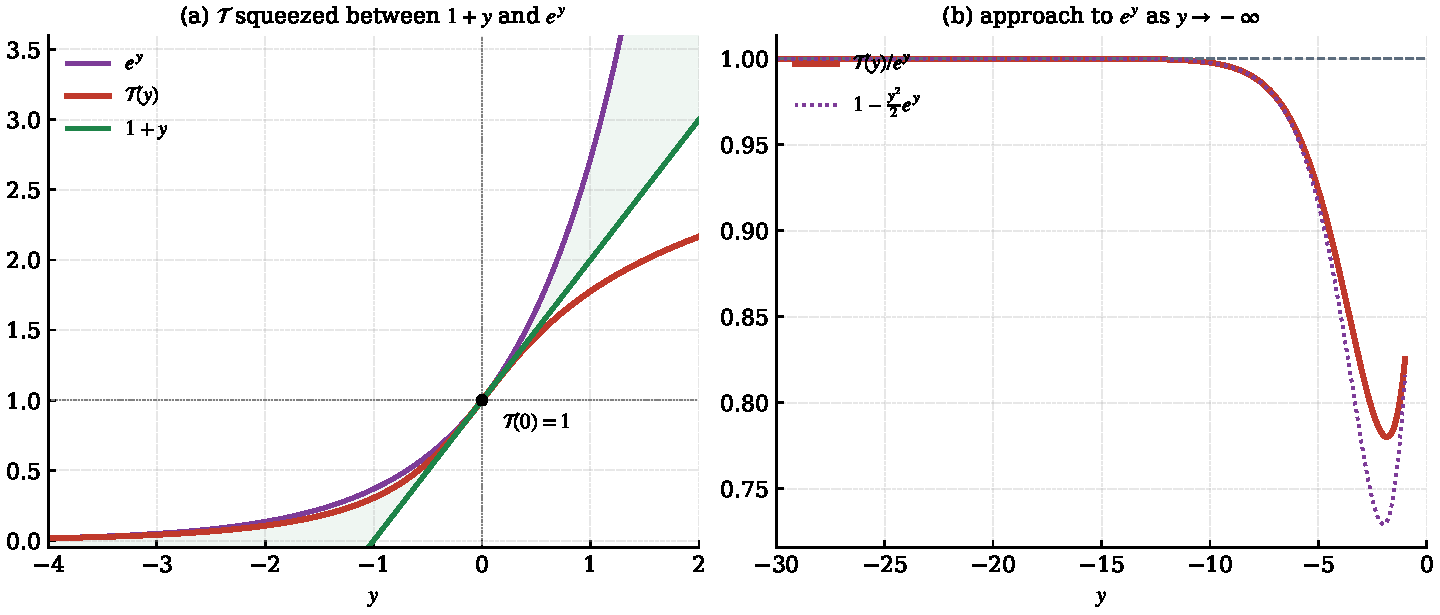
\includegraphics[width=0.98\textwidth]{figures/fig2_sandwich.pdf}
    \caption{(a) The sandwich of Theorem~\ref{thm:sandwich}: on
    $(-1,0)$, $1+y < \Tah(y) < \ee^{y}$ (shaded strip); for $y > 0$,
    $\Tah(y) < 1 + y < \ee^{y}$. (b) The ratio $\Tah(y)/\ee^{y}$
    (solid) against the asymptotic prediction
    $1 - \tfrac{y^{2}}{2}\ee^{y}$ of Theorem~\ref{thm:asymptotics}
    (dotted): the Tahawus function is an asymptotic copy of $\exp$
    on the far left.}
    \label{fig:sandwich}
\end{figure}

The exponential comparison can be sharpened to a Lipschitz statement:
the slope of $\Tah$ never exceeds $1$.

\begin{proposition}[$1$-Lipschitz property]\label{prop:lipschitz}
For all $y \in \R$,
\[
    0 \;<\; \Tah'(y) \;\le\; 1 ,
    \qquad\text{with equality iff } y = 0 .
\]
Equivalently, $f'(x) \ge 1$ for all $x > 0$ with equality only at
$x = 1$; hence $|\Tah(y_{1}) - \Tah(y_{2})| \le |y_{1} - y_{2}|$ for all
real $y_{1}, y_{2}$.
\end{proposition}

\begin{proof}
By \eqref{eq:x2fprime},
$x^{2}(f'(x) - 1) = h(x) := x^{x}(x\ln x + x - 1) + 1 - x^{2}$, so we
must show $h \ge 0$ on $(0,\infty)$ with equality only at $x = 1$. Put
$a := x \ln x$ and $m := x\ln x + x - 1 = a + x - 1$.

\emph{Case $x \ge 1$.} Then $a \ge 0$ and $m \ge 0$ (as $m(1) = 0$ and
$m' = \ln x + 2 > 0$ on $[1,\infty)$). Since $\ee^{a} \ge 1 + a$,
\[
    h \;\ge\; (1 + a)(a + x - 1) + 1 - x^{2}
    \;=\; x^{2}\ln x\,(\ln x + 1) + x - x^{2}
    \;=\; x\,p(x),
\]
where $p(x) := x\ln x\,(\ln x + 1) - x + 1$. Now
$p(1) = 0$ and $p'(x) = \ln x\,(\ln x + 3) \ge 0$ for $x \ge 1$, so
$p \ge 0$ on $[1,\infty)$, hence $h \ge 0$; equality forces $a = 0$
(i.e.\ $x = 1$) and $p(x) = 0$.

\emph{Case $0 < x < 1$.} Then $m < 0$ (as $m$ decreases from
$-1$ at $0^{+}$, has its minimum $-\ee^{-2} - 1 < 0$ at $x = \ee^{-2}$,
and returns to $m(1) = 0$ only at the endpoint). Since
$u := a = x\ln x \in (-\tfrac1\ee, 0)$ and $\ee^{u} \le \tfrac{1}{1-u}$
(the inequality $\ee^{-u} \ge 1 - u$ for $u < 1$), and since $m < 0$,
\[
    x^{x} m \;=\; \ee^{u}\,m \;\ge\; \frac{m}{1 - u} .
\]
Therefore
\[
    h \;\ge\; \frac{m}{1 - x\ln x} + 1 - x^{2}
    \;=\; \frac{x - x^{2} + x^{3}\ln x}{1 - x\ln x}
    \;=\; \frac{x\,r(x)}{1 - x\ln x},
\]
where $r(x) := 1 - x + x^{2}\ln x$. The denominator exceeds $1$, and
$r > 0$ on $(0,1)$: indeed $r(1) = 0$, $r(0^{+}) = 1$, and
$r'(x) = x(1 + 2\ln x) - 1 < 0$ on $(0,1)$ because the auxiliary
function $u_{1}(x) := x(1 + 2\ln x)$ satisfies $u_{1} \le 1$ on
$(0,1]$, with equality only at $x = 1$ (Lemma~\ref{lem:u1} in the
Appendix). Hence $r$ decreases strictly from $1$
to $0$ and is positive. This gives $h > 0$ on $(0,1)$, completing the
proof.
\end{proof}

\begin{remark}
Proposition~\ref{prop:lipschitz} says that $\Tah$ is a (weak)
contraction of the whole real line into the positive half-line. In
particular the graph of $\Tah$ is flatter than the diagonal everywhere
except at the origin, where it is tangent to it; this is visible in
Figure~\ref{fig:mirror} and is the mechanism behind the global dynamics
of Section~\ref{sec:dynamics}. Note the pleasing division of labour in
the proof: the elementary inequalities $\ee^{u} \ge 1 + u$ (for $u \ge
0$) and $\ee^{u} \le 1/(1-u)$ (for $u < 1$) each take care of one side
of $x = 1$.
\end{remark}
